\documentclass[twoside]{book}

% Packages required by doxygen
\usepackage{fixltx2e}
\usepackage{calc}
\usepackage{doxygen}
\usepackage[export]{adjustbox} % also loads graphicx
\usepackage{graphicx}
\usepackage[utf8]{inputenc}
\usepackage{makeidx}
\usepackage{multicol}
\usepackage{multirow}
\PassOptionsToPackage{warn}{textcomp}
\usepackage{textcomp}
\usepackage[nointegrals]{wasysym}
\usepackage[table]{xcolor}

% Font selection
\usepackage[T1]{fontenc}
\usepackage[scaled=.90]{helvet}
\usepackage{courier}
\usepackage{amssymb}
\usepackage{sectsty}
\renewcommand{\familydefault}{\sfdefault}
\allsectionsfont{%
  \fontseries{bc}\selectfont%
  \color{darkgray}%
}
\renewcommand{\DoxyLabelFont}{%
  \fontseries{bc}\selectfont%
  \color{darkgray}%
}
\newcommand{\+}{\discretionary{\mbox{\scriptsize$\hookleftarrow$}}{}{}}

% Page & text layout
\usepackage{geometry}
\geometry{%
  a4paper,%
  top=2.5cm,%
  bottom=2.5cm,%
  left=2.5cm,%
  right=2.5cm%
}
\tolerance=750
\hfuzz=15pt
\hbadness=750
\setlength{\emergencystretch}{15pt}
\setlength{\parindent}{0cm}
\setlength{\parskip}{3ex plus 2ex minus 2ex}
\makeatletter
\renewcommand{\paragraph}{%
  \@startsection{paragraph}{4}{0ex}{-1.0ex}{1.0ex}{%
    \normalfont\normalsize\bfseries\SS@parafont%
  }%
}
\renewcommand{\subparagraph}{%
  \@startsection{subparagraph}{5}{0ex}{-1.0ex}{1.0ex}{%
    \normalfont\normalsize\bfseries\SS@subparafont%
  }%
}
\makeatother

% Headers & footers
\usepackage{fancyhdr}
\pagestyle{fancyplain}
\fancyhead[LE]{\fancyplain{}{\bfseries\thepage}}
\fancyhead[CE]{\fancyplain{}{}}
\fancyhead[RE]{\fancyplain{}{\bfseries\leftmark}}
\fancyhead[LO]{\fancyplain{}{\bfseries\rightmark}}
\fancyhead[CO]{\fancyplain{}{}}
\fancyhead[RO]{\fancyplain{}{\bfseries\thepage}}
\fancyfoot[LE]{\fancyplain{}{}}
\fancyfoot[CE]{\fancyplain{}{}}
\fancyfoot[RE]{\fancyplain{}{\bfseries\scriptsize Generated by Doxygen }}
\fancyfoot[LO]{\fancyplain{}{\bfseries\scriptsize Generated by Doxygen }}
\fancyfoot[CO]{\fancyplain{}{}}
\fancyfoot[RO]{\fancyplain{}{}}
\renewcommand{\footrulewidth}{0.4pt}
\renewcommand{\chaptermark}[1]{%
  \markboth{#1}{}%
}
\renewcommand{\sectionmark}[1]{%
  \markright{\thesection\ #1}%
}

% Indices & bibliography
\usepackage{natbib}
\usepackage[titles]{tocloft}
\setcounter{tocdepth}{3}
\setcounter{secnumdepth}{5}
\makeindex

% Hyperlinks (required, but should be loaded last)
\usepackage{ifpdf}
\ifpdf
  \usepackage[pdftex,pagebackref=true]{hyperref}
\else
  \usepackage[ps2pdf,pagebackref=true]{hyperref}
\fi
\hypersetup{%
  colorlinks=true,%
  linkcolor=blue,%
  citecolor=blue,%
  unicode%
}

% Custom commands
\newcommand{\clearemptydoublepage}{%
  \newpage{\pagestyle{empty}\cleardoublepage}%
}

\usepackage{caption}
\captionsetup{labelsep=space,justification=centering,font={bf},singlelinecheck=off,skip=4pt,position=top}

%===== C O N T E N T S =====

\begin{document}

% Titlepage & ToC
\hypersetup{pageanchor=false,
             bookmarksnumbered=true,
             pdfencoding=unicode
            }
\pagenumbering{alph}
\begin{titlepage}
\vspace*{7cm}
\begin{center}%
{\Large hangmansolver }\\
\vspace*{1cm}
{\large Generated by Doxygen 1.8.13}\\
\end{center}
\end{titlepage}
\clearemptydoublepage
\pagenumbering{roman}
\tableofcontents
\clearemptydoublepage
\pagenumbering{arabic}
\hypersetup{pageanchor=true}

%--- Begin generated contents ---
\chapter{Welcome to lib\+\_\+hangman}
\label{index}\hypertarget{index}{}\hypertarget{index_intro_sec}{}\section{Introduction}\label{index_intro_sec}
This is a collection of functions designed to help you build a crossword / hangman game / solver.\hypertarget{index_usage}{}\section{Usage}\label{index_usage}
See the \hyperlink{unhangman_8h}{include/unhangman.\+h} in the files tab. 
\chapter{File Index}
\section{File List}
Here is a list of all documented files with brief descriptions\+:\begin{DoxyCompactList}
\item\contentsline{section}{include/\hyperlink{unhangman_8h}{unhangman.\+h} \\*Declarations of all the functions }{\pageref{unhangman_8h}}{}
\item\contentsline{section}{src/\hyperlink{unhangman_8cpp}{unhangman.\+cpp} \\*Implementations of all the functions }{\pageref{unhangman_8cpp}}{}
\end{DoxyCompactList}

\chapter{File Documentation}
\hypertarget{hangman_8h}{}\section{include/hangman.h File Reference}
\label{hangman_8h}\index{include/hangman.\+h@{include/hangman.\+h}}


Declarations of all the functions.  


{\ttfamily \#include $<$vector$>$}\\*
{\ttfamily \#include $<$map$>$}\\*
{\ttfamily \#include $<$experimental/optional$>$}\\*
{\ttfamily \#include $<$algorithm$>$}\\*
Include dependency graph for hangman.\+h\+:
\nopagebreak
\begin{figure}[H]
\begin{center}
\leavevmode
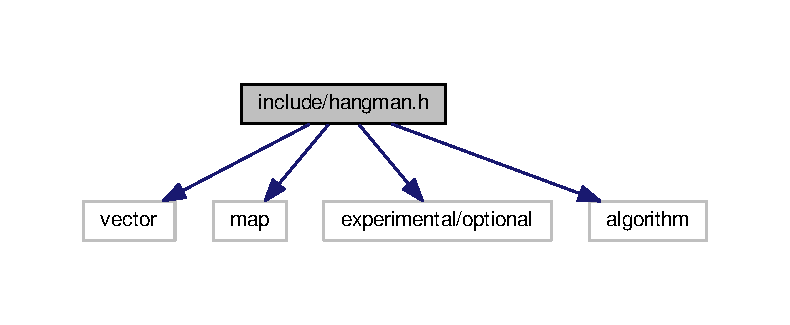
\includegraphics[width=350pt]{hangman_8h__incl}
\end{center}
\end{figure}
This graph shows which files directly or indirectly include this file\+:
\nopagebreak
\begin{figure}[H]
\begin{center}
\leavevmode
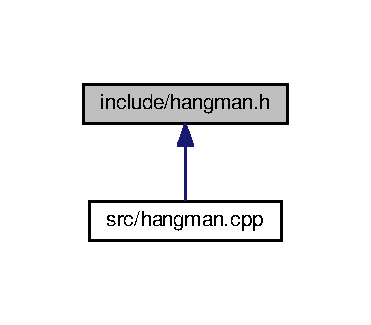
\includegraphics[width=178pt]{hangman_8h__dep__incl}
\end{center}
\end{figure}
\subsection*{Functions}
\begin{DoxyCompactItemize}
\item 
std\+::vector$<$ std\+::string $>$ {\bfseries read\+\_\+dictionary} (const std\+::string \&path)\hypertarget{hangman_8h_ada47e9338f9e87b423f8214dc4a736e6}{}\label{hangman_8h_ada47e9338f9e87b423f8214dc4a736e6}

\item 
std\+::vector$<$ std\+::string $>$ {\bfseries filter\+\_\+length} (const std\+::vector$<$ std\+::string $>$ \&dictionary, unsigned length)\hypertarget{hangman_8h_a4905d4615c76e8b03b2485034f1dbda1}{}\label{hangman_8h_a4905d4615c76e8b03b2485034f1dbda1}

\item 
std\+::vector$<$ std\+::string $>$ {\bfseries filter\+\_\+pattern} (const std\+::vector$<$ std\+::string $>$ \&dictionary, const std\+::string \&pattern, char wildcard= \textquotesingle{}$\ast$\textquotesingle{})\hypertarget{hangman_8h_a60affe8873225d408834b4bacee2461e}{}\label{hangman_8h_a60affe8873225d408834b4bacee2461e}

\item 
std\+::map$<$ char, unsigned $>$ {\bfseries count\+\_\+character\+\_\+frequency} (const std\+::vector$<$ std\+::string $>$ \&dictionary, const std\+::string \&pattern=\char`\"{}\char`\"{})\hypertarget{hangman_8h_a1622b1d311b2495ae299f8c875a5573d}{}\label{hangman_8h_a1622b1d311b2495ae299f8c875a5573d}

\item 
std\+::vector$<$ char $>$ {\bfseries frequency\+\_\+to\+\_\+array} (const std\+::map$<$ char, unsigned $>$ \&character\+\_\+frequency)\hypertarget{hangman_8h_a3663781c1785f8bd725da940b07e2fb9}{}\label{hangman_8h_a3663781c1785f8bd725da940b07e2fb9}

\item 
std\+::experimental\+::optional$<$ char $>$ {\bfseries get\+\_\+next\+\_\+char} (const std\+::vector$<$ char $>$ \&char\+\_\+array, const std\+::string \&ignore=\char`\"{}\char`\"{})\hypertarget{hangman_8h_ac09e771692a2604aa55d5675a3802fd2}{}\label{hangman_8h_ac09e771692a2604aa55d5675a3802fd2}

\item 
std\+::experimental\+::optional$<$ char $>$ {\bfseries get\+\_\+next\+\_\+vowel} (const std\+::vector$<$ char $>$ \&char\+\_\+array, const std\+::string \&ignore=\char`\"{}\char`\"{})\hypertarget{hangman_8h_a75083dc0d9702a9641461d8a4c14bbca}{}\label{hangman_8h_a75083dc0d9702a9641461d8a4c14bbca}

\item 
std\+::experimental\+::optional$<$ char $>$ {\bfseries get\+\_\+next\+\_\+constant} (const std\+::vector$<$ char $>$ \&char\+\_\+array, const std\+::string \&ignore=\char`\"{}\char`\"{})\hypertarget{hangman_8h_a223617d2b5703642d65670e7f49d2a5e}{}\label{hangman_8h_a223617d2b5703642d65670e7f49d2a5e}

\item 
std\+::experimental\+::optional$<$ std\+::vector$<$ unsigned $>$ $>$ {\bfseries find\+\_\+char\+\_\+positions} (const std\+::vector$<$ std\+::string $>$ \&dictionary, char c)\hypertarget{hangman_8h_a8b79ef16e04c4f46d2204a618a3b6fb9}{}\label{hangman_8h_a8b79ef16e04c4f46d2204a618a3b6fb9}

\item 
std\+::string \hyperlink{hangman_8h_a42afc8ba3705f150db1712c2f4e35f0c}{remove\+\_\+pattern} (const std\+::string \&word, const std\+::string \&pattern, char wildcard= \textquotesingle{}$\ast$\textquotesingle{})
\begin{DoxyCompactList}\small\item\em Removes the characters of pattern from word. \end{DoxyCompactList}\item 
std\+::vector$<$ std\+::string $>$ \hyperlink{hangman_8h_a57fca433ea4c6ee0693e612668c383e4}{must\+\_\+contain} (const std\+::vector$<$ std\+::string $>$ \&dictionary, char c, const std\+::string \&pattern=\char`\"{}\char`\"{})
\begin{DoxyCompactList}\small\item\em Returns a vector of words that contain the specified character, ignoring it\textquotesingle{}s appearence in the pattern (if provided) \end{DoxyCompactList}\item 
std\+::vector$<$ std\+::string $>$ \hyperlink{hangman_8h_aa0d9948dada05cb5694dae370b69fc0b}{must\+\_\+not\+\_\+contain} (const std\+::vector$<$ std\+::string $>$ \&dictionary, char c, const std\+::string \&pattern=\char`\"{}\char`\"{})
\begin{DoxyCompactList}\small\item\em Returns a vector of words that don\textquotesingle{}t contain the specified character, ignoring it\textquotesingle{}s appearence in the pattern (if provided) \end{DoxyCompactList}\end{DoxyCompactItemize}


\subsection{Detailed Description}
Declarations of all the functions. 



\subsection{Function Documentation}
\index{hangman.\+h@{hangman.\+h}!must\+\_\+contain@{must\+\_\+contain}}
\index{must\+\_\+contain@{must\+\_\+contain}!hangman.\+h@{hangman.\+h}}
\subsubsection[{\texorpdfstring{must\+\_\+contain(const std\+::vector$<$ std\+::string $>$ \&dictionary, char c, const std\+::string \&pattern="""")}{must_contain(const std::vector< std::string > &dictionary, char c, const std::string &pattern="")}}]{\setlength{\rightskip}{0pt plus 5cm}std\+::vector$<$std\+::string$>$ must\+\_\+contain (
\begin{DoxyParamCaption}
\item[{const std\+::vector$<$ std\+::string $>$ \&}]{dictionary, }
\item[{char}]{c, }
\item[{const std\+::string \&}]{pattern}
\end{DoxyParamCaption}
)}\hypertarget{hangman_8h_a57fca433ea4c6ee0693e612668c383e4}{}\label{hangman_8h_a57fca433ea4c6ee0693e612668c383e4}


Returns a vector of words that contain the specified character, ignoring it\textquotesingle{}s appearence in the pattern (if provided) 


\begin{DoxyParams}{Parameters}
{\em dictionary} & A vector of words that you are currently choosing from \\
\hline
{\em c} & The character that the words must contain \\
\hline
{\em pattern} & The pattern wich should be ignored in all words\\
\hline
\end{DoxyParams}
\begin{DoxyReturn}{Returns}
a vector of words that contain the specified character. 
\end{DoxyReturn}
\index{hangman.\+h@{hangman.\+h}!must\+\_\+not\+\_\+contain@{must\+\_\+not\+\_\+contain}}
\index{must\+\_\+not\+\_\+contain@{must\+\_\+not\+\_\+contain}!hangman.\+h@{hangman.\+h}}
\subsubsection[{\texorpdfstring{must\+\_\+not\+\_\+contain(const std\+::vector$<$ std\+::string $>$ \&dictionary, char c, const std\+::string \&pattern="""")}{must_not_contain(const std::vector< std::string > &dictionary, char c, const std::string &pattern="")}}]{\setlength{\rightskip}{0pt plus 5cm}std\+::vector$<$std\+::string$>$ must\+\_\+not\+\_\+contain (
\begin{DoxyParamCaption}
\item[{const std\+::vector$<$ std\+::string $>$ \&}]{dictionary, }
\item[{char}]{c, }
\item[{const std\+::string \&}]{pattern}
\end{DoxyParamCaption}
)}\hypertarget{hangman_8h_aa0d9948dada05cb5694dae370b69fc0b}{}\label{hangman_8h_aa0d9948dada05cb5694dae370b69fc0b}


Returns a vector of words that don\textquotesingle{}t contain the specified character, ignoring it\textquotesingle{}s appearence in the pattern (if provided) 


\begin{DoxyParams}{Parameters}
{\em dictionary} & A vector of words that you are currently choosing from \\
\hline
{\em c} & The character that the words must not contain \\
\hline
{\em pattern} & The pattern wich should be ignored in all words\\
\hline
\end{DoxyParams}
\begin{DoxyReturn}{Returns}
a vector of words that don\textquotesingle{}t contain the specified character. 
\end{DoxyReturn}
\index{hangman.\+h@{hangman.\+h}!remove\+\_\+pattern@{remove\+\_\+pattern}}
\index{remove\+\_\+pattern@{remove\+\_\+pattern}!hangman.\+h@{hangman.\+h}}
\subsubsection[{\texorpdfstring{remove\+\_\+pattern(const std\+::string \&word, const std\+::string \&pattern, char wildcard= \textquotesingle{}$\ast$\textquotesingle{})}{remove_pattern(const std::string &word, const std::string &pattern, char wildcard= '*')}}]{\setlength{\rightskip}{0pt plus 5cm}std\+::string remove\+\_\+pattern (
\begin{DoxyParamCaption}
\item[{const std\+::string \&}]{word, }
\item[{const std\+::string \&}]{pattern, }
\item[{char}]{wildcard}
\end{DoxyParamCaption}
)}\hypertarget{hangman_8h_a42afc8ba3705f150db1712c2f4e35f0c}{}\label{hangman_8h_a42afc8ba3705f150db1712c2f4e35f0c}


Removes the characters of pattern from word. 


\begin{DoxyParams}{Parameters}
{\em word} & The word you need to clean up \\
\hline
{\em pattern} & The characters you want removed from word \\
\hline
{\em wildcard} & If this character is in the pattern it will not be removed from word\\
\hline
\end{DoxyParams}
\begin{DoxyReturn}{Returns}
The word but without any characters of the pattern 
\end{DoxyReturn}

\hypertarget{hangmansolver_8cpp}{}\section{src/hangmansolver.cpp File Reference}
\label{hangmansolver_8cpp}\index{src/hangmansolver.\+cpp@{src/hangmansolver.\+cpp}}


Implementations of all the functions.  


{\ttfamily \#include $<$iterator$>$}\newline
{\ttfamily \#include $<$algorithm$>$}\newline
{\ttfamily \#include $<$fstream$>$}\newline
{\ttfamily \#include \char`\"{}../include/hangman.\+h\char`\"{}}\newline
Include dependency graph for hangmansolver.\+cpp\+:

%--- End generated contents ---

% Index
\backmatter
\newpage
\phantomsection
\clearemptydoublepage
\addcontentsline{toc}{chapter}{Index}
\printindex

\end{document}
